% RASD for the loading update of PoliVerse. Build: scripts/docs.sh
\documentclass[rasd]{se2doc}
% Written once per project; every document reads it.
% Each document sets its own \docversion and \revision lines after reading this.
\project{PoliVerse Loading Update}
\authors{Samuele Segrini}
\docdate{10 November 2026}

\docversion{1.0}
\revision{0.1}{10 Nov 2026}{First draft: goals, assumptions, requirements and use cases}
\revision{1.0}{10 Nov 2026}{Requirements agreed; Alloy model added to section 4}
% Domain terms, shared by every document.
\term{Screen}{One page of the app the student opens, such as Carriera or Aule libere.}
\term{Section}{A titled block of a screen that can be read on its own, such as the libretto inside Carriera.}
\term{Part}{The data behind one section: the answer to one request, or to one group of requests that only make sense together.}
\term{Stored copy}{A part kept on the phone from an earlier load, with the time it was fetched.}
\term{Max age}{How long a stored copy of a given kind of part is shown without asking the server again.}
\term{First content}{The first section of a screen that shows real data after the student opens it.}
\term{Speculative request}{A request the student did not ask for by opening a screen: a prefetch or an offline pack request.}
\term{Prefetch}{Fetching a part before the student opens the screen that shows it.}
\term{Offline pack}{The set of parts fetched ahead so that the app works with no connection.}
\term{Reveal}{The short animation with which arriving content writes itself onto the screen.}
\term{Loading ledger}{The on-device record of how long each part took and whether a speculative request was used.}
\term{Booking boundary}{A moment at which a room's booking starts or ends, so that the room changes between free and occupied.}
\term{Host}{One server of the Politecnico the app talks to, such as \texttt{api.polimi.it}.}
\term{Baseline}{The measurement taken with the loading ledger on the build before a change.}

\usetikzlibrary{positioning,arrows.meta,shapes.multipart,fit}

% Values marked with a dagger are initial values, see section 1.3.
\newcommand\initial{\textsuperscript{\dag}}

\begin{document}
\maketitle

% DRAFT, rewrite
\section{Introduction}

\subsection{Purpose}
PoliVerse is an unofficial app for students of the Politecnico di Milano. It shows
courses, materials, the timetable, the career and the campus in one place. This
document specifies one update to it: how the app loads data and how it shows data
that is still on its way.

Today several screens wait for every request to answer before showing anything, the
app cannot tell ``empty'' from ``not here yet'', and nothing is prepared before the
student asks for it. The update serves the following goals.

\goal{G1}{A student who opens a screen sees its first useful content without waiting for everything on that screen.}
\goal{G2}{A student is never shown a statement or a number that is false only because data is still on its way.}
\goal{G3}{A student who is about to attend a lecture finds what they need for it already on the phone.}
\goal{G4}{A student can consult the timetable, the campus, the rooms and their courses with no network connection.}
\goal{G5}{A student notices what changed since they last looked without reading everything again.}
\goal{G6}{Work the student did not ask for never spends their mobile data or battery beyond what they allowed, and stays within a fixed number of requests to the Politecnico.}
\goal{G7}{The developer can tell from measurements taken on a phone whether a change to loading helped.}

\subsection{Scope}
The machine is the PoliVerse app on iPhone, with its widgets and background tasks.
The world is the student, the phone and its network, and the Politecnico's servers.
The project runs no server of its own.

\begin{center}\small
\begin{tabularx}{\linewidth}{@{}X l@{}}
  \toprule
  Phenomenon & Kind \\
  \midrule
  A lecture takes place in a room at a given time & World \\
  A room is booked or a booking is withdrawn & World \\
  A grade is published, an exam sitting opens, a lecture is moved & World \\
  The student travels through a place with no signal & World \\
  The student opens a screen, scrolls, taps a retry control & Shared, world controlled \\
  A server answers a request, fails, or does not answer & Shared, world controlled \\
  The network becomes available, metered or unavailable & Shared, world controlled \\
  iOS grants background time; reports Low Data Mode, Low Power Mode and heat & Shared, world controlled \\
  The app sends a request to a server & Shared, machine controlled \\
  The app shows, updates or animates a section & Shared, machine controlled \\
  The app delivers a local notification or a haptic & Shared, machine controlled \\
  The app keeps a stored copy, orders requests, records the ledger & Machine \\
  \bottomrule
\end{tabularx}
\end{center}

In scope: showing sections as their parts arrive, the order of requests, storing and
ageing parts one by one, deadlines for slow parts, prefetching from the timetable, an
offline pack, refreshing at booking boundaries, noticing changes, the limits on
speculative requests, and the loading ledger.

Out of scope: any server operated by the project and therefore real push; predicting
the next screen from the student's habits; changes to what the screens contain;
loading of recordings' video, which has its own download manager.

\subsection{Definitions, acronyms, abbreviations}
\printterms

\noindent Acronyms: RASD, Requirements Analysis and Specification Document; DD, Design
Document; UC, use case; HIG, Human Interface Guidelines; TTL, time to live.

\noindent A number followed by \initial{} is an initial value. It is a requirement as
written, and it is confirmed or changed once the loading ledger (\idref{R34}) has
produced a baseline.

\subsection{Revision history}
See the table under the title.

\subsection{Reference documents}
Listed in section 6.

\subsection{Document structure}
Section 2 describes the update from the outside: scenarios, the domain, the
functions, the users and the assumptions about the world. Section 3 lists the
requirements: interfaces, functional requirements with their use cases, performance
requirements, constraints and system attributes. Section 4 states what is checked
formally. Sections 5 and 6 hold the effort spent and the references.

% DRAFT, rewrite
\section{Overall description}

\subsection{Product perspective}

\subsubsection{Scenarios}

\paragraph{S1, first sign-in.} Giulia installs PoliVerse and signs in. Carriera needs
six answers from the Politecnico. The libretto answers first and writes itself onto
the screen while the exam sittings are still loading. Their section shows its title
and a waiting line, not ``Nessun appello''. The weighted average stays hidden until
the credits counter has arrived, then appears once with its final value.

\paragraph{S2, a free room between lectures.} Marco leaves a lecture in building 3 and
opens Aule libere. The rooms of the buildings on his map are asked first, so the
first free rooms listed are a short walk away. The rest of the campus fills in
below without moving what he is reading.

\paragraph{S3, the lecture is ready.} At 9:05 Sara has a lecture at 9:15 in a room she
has never been to. When she opens the app in the corridor, the room, its floor plan
and the building's 3D model appear at once, because the app fetched them when it
last ran.

\paragraph{S4, no signal.} Luca is on the metro with no connection. He opens the
timetable, tomorrow's free rooms and a course page. Each shows its stored copy with
its age, and no error covers the screen. In Impostazioni he can see what is ready
offline.

\paragraph{S5, a slow server.} One career endpoint does not answer. After four
seconds its section shows the copy from this morning, marked with its age, while the
other sections are fresh. The app keeps trying in the background and replaces the
copy when the answer comes.

\paragraph{S6, a new grade.} A grade is published in the afternoon. The next time the
app refreshes, in the background or when Anna opens it, it notices the new row. Anna
gets a notification, and in the libretto only that row writes itself in and is
marked as new.

\subsubsection{Domain model}
A screen is made of sections. Each section shows one part. A part is fetched by one
or more requests to a host and may have a stored copy on the phone. The class
diagram shows the terms, and the state diagram shows the life of a section while its
screen is open.

\begin{figure}[h]
\centering
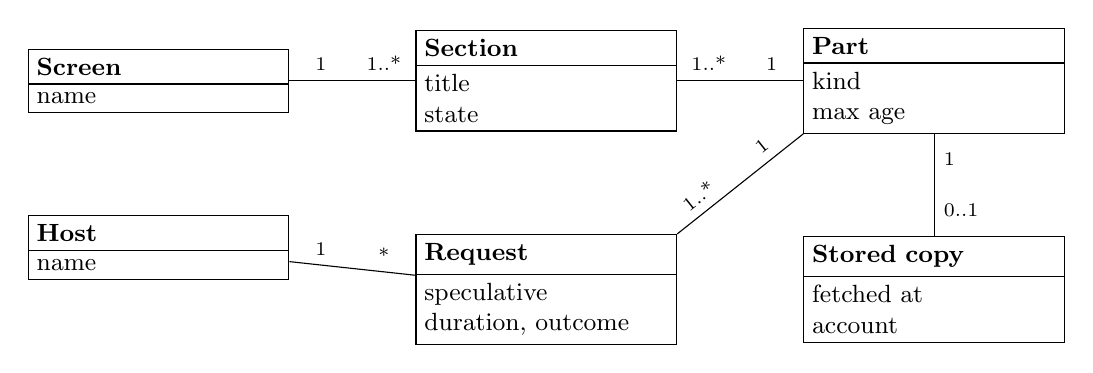
\begin{tikzpicture}[
  class/.style={draw, rectangle split, rectangle split parts=2, align=left,
    font=\small, text width=3.1cm, inner sep=3pt},
  rel/.style={-, thin}, lab/.style={font=\scriptsize}]
  \node[class] (screen) {\textbf{Screen}\nodepart{two}name};
  \node[class, right=1.6cm of screen] (section) {\textbf{Section}\nodepart{two}title\\state};
  \node[class, right=1.6cm of section] (part) {\textbf{Part}\nodepart{two}kind\\max age};
  \node[class, below=1.3cm of part] (copy) {\textbf{Stored copy}\nodepart{two}fetched at\\account};
  \node[class, below=1.3cm of section] (request) {\textbf{Request}\nodepart{two}speculative\\duration, outcome};
  \node[class, below=1.3cm of screen] (host) {\textbf{Host}\nodepart{two}name};
  \draw[rel] (screen) -- node[lab, above, near start]{1} node[lab, above, near end]{1..*} (section);
  \draw[rel] (section) -- node[lab, above, near start]{1..*} node[lab, above, near end]{1} (part);
  \draw[rel] (part) -- node[lab, right, near start]{1} node[lab, right, near end]{0..1} (copy);
  \draw[rel] (part.south west) -- node[lab, above, sloped, near start]{1} node[lab, above, sloped, near end]{1..*} (request.north east);
  \draw[rel] (request) -- node[lab, above, near start]{*} node[lab, above, near end]{1} (host);
\end{tikzpicture}
\caption{Domain model of loading.}
\end{figure}

\begin{figure}[h]
\centering
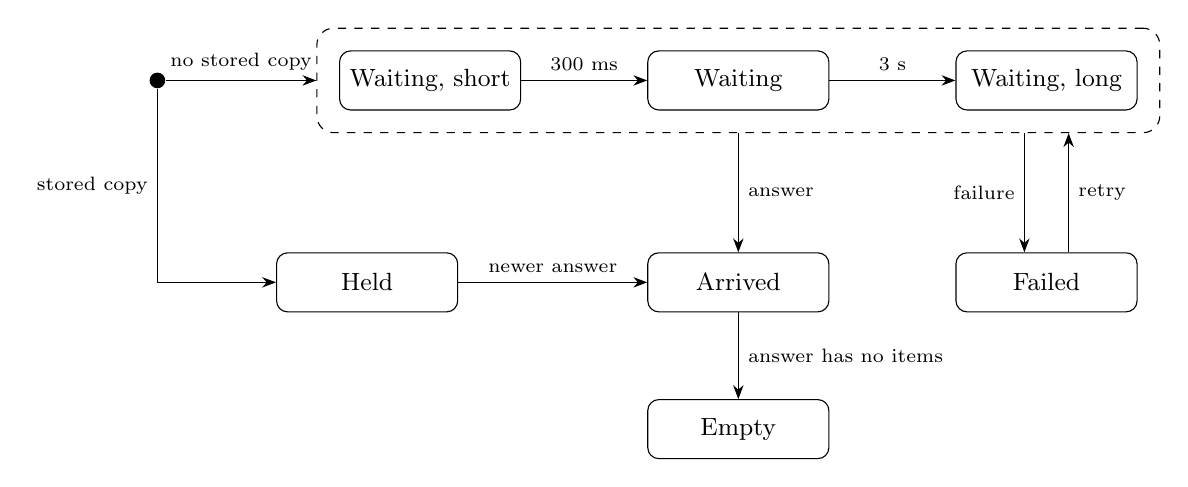
\begin{tikzpicture}[
  st/.style={draw, rounded corners=4pt, font=\small, minimum height=0.75cm,
    minimum width=2.3cm, align=center},
  tr/.style={-{Stealth[length=5pt]}, thin}, lab/.style={font=\scriptsize, align=center}]
  \node[st] (short) {Waiting, short};
  \node[st, right=1.6cm of short] (wait) {Waiting};
  \node[st, right=1.6cm of wait] (long) {Waiting, long};
  \node[draw, dashed, rounded corners=6pt, inner sep=8pt, fit=(short)(wait)(long)] (box) {};
  \node[st, below=1.8cm of wait] (arrived) {Arrived};
  \node[st, left=2.4cm of arrived] (held) {Held};
  \node[st, right=1.6cm of arrived] (failed) {Failed};
  \node[st, below=1.1cm of arrived] (empty) {Empty};
  \node[circle, fill, inner sep=2pt, left=2.2cm of short] (start) {};
  \draw[tr] (start) -- node[lab, above]{no stored copy} (box.west);
  \draw[tr] (start) |- node[lab, left, pos=0.25]{stored copy} (held.west);
  \draw[tr] (short) -- node[lab, above]{300 ms} (wait);
  \draw[tr] (wait) -- node[lab, above]{3 s} (long);
  \draw[tr] (box.south) -- node[lab, right]{answer} (arrived);
  \draw[tr] ([xshift=-8pt]box.south -| failed) -- node[lab, left]{failure} ([xshift=-8pt]failed.north);
  \draw[tr] ([xshift=8pt]failed.north) -- node[lab, right]{retry} ([xshift=8pt]box.south -| failed);
  \draw[tr] (held) -- node[lab, above]{newer answer} (arrived);
  \draw[tr] (arrived) -- node[lab, right]{answer has no items} (empty);
\end{tikzpicture}
\caption{States of a section while its screen is open. A failure with a stored copy leaves the section in Held.}
\end{figure}

\subsection{Product functions}
\begin{description}[style=nextline, leftmargin=1.5em]
  \item[F1, partial display] Each section appears when its part arrives, in one of seven states, with one shared look for waiting, arriving, empty and failed.
  \item[F2, relevance order] Requests of a screen that needs many are sent in the order of what the student is looking at.
  \item[F3, parts stored and aged one by one] Each part is kept as soon as it arrives and has its own max age, so a load resumes and a refresh asks only for what is old.
  \item[F4, part deadlines] A slow part stops holding its section: the stored copy stands in and the app retries.
  \item[F5, timetable prefetch] What a lecture needs is fetched before it starts.
  \item[F6, offline pack] A defined set of parts is fetched ahead and its readiness is shown.
  \item[F7, boundary refresh] Free rooms stay correct as bookings start and end, without polling.
  \item[F8, change awareness] The app knows what changed in a refresh, marks it, and can notify.
  \item[F9, speculative budget] Prefetch and offline pack obey limits on data, power and requests.
  \item[F10, loading ledger] Every load is timed on the device and reported.
\end{description}

\subsection{User characteristics}
\begin{description}[style=nextline, leftmargin=1.5em]
  \item[Student] Enrolled at the Politecnico, signed in with their own account. Uses the app in short visits between lectures, often on mobile data and sometimes with no signal. Does not know and should not need to know which data comes from which server.
  \item[Developer] The one developer of the app. Reads the loading ledger on their own phone to decide what to change next.
\end{description}

\subsection{Assumptions, dependencies and constraints}
\assumption{D1}{A server of the Politecnico answers each request with one whole response; it never sends a response in usable pieces.}
\assumption{D2}{The Politecnico's servers send no cache validators and offer no push, subscription or change feed (measured on 12 September 2026).}
\assumption{D3}{Some screens need several requests: the career needs six, the free rooms of a campus need one per room, up to 158, and a course page needs three in a row.}
\assumption{D4}{A request is usually answered in 0.2 to 3 seconds, and occasionally not until a timeout of about 15 seconds.}
\assumption{D5}{The student's timetable is known days ahead, and a lecture takes place in the room and at the time the timetable states.}
\assumption{D6}{The bookings of a room for a given day rarely change during that day.}
\assumption{D7}{iOS decides whether and when a background task runs. A refresh task gets at most 30 seconds; a processing task runs only when the system chooses, typically while charging.}
\assumption{D8}{iOS reports truthfully whether the network is unavailable, metered or in Low Data Mode, and whether the phone is in Low Power Mode or hot.}
\assumption{D9}{Students regularly pass through places with no connection, such as the metro.}
\assumption{D10}{The data a server returns for a signed-in account belongs to that student, and each item in it can be told apart from the others by a stable identity such as an exam code or a lecture's id.}
\assumption{D11}{The Politecnico tolerates the request volume of an unofficial client as long as it stays close to what a person using the official services would cause.}

\noindent Dependencies, all already in the app: the store layer (\texttt{Resource},
\texttt{Loader}, \texttt{Query}, \texttt{OfflineStore}), the warm-up and scroll
prefetch, the freshness coordinator, the device pressure and network monitors, the
exam update feed and the diagnostics report.

% DRAFT, rewrite
\section{Specific requirements}

\subsection{External interface requirements}

\subsubsection{User interfaces}
Every section of a screen is in exactly one of the states of the state diagram in
section 2.1.2, and each state has one look, shared by all screens:
\begin{itemize}
  \item Held: the content, with no indicator over it.
  \item Waiting, short: the section's space, empty.
  \item Waiting: the section's title and one soft waiting line where the first line of text will be. No grey placeholder blocks.
  \item Waiting, long: the same, plus one line naming the step in progress or a count.
  \item Arrived: the content writes itself in with the reveal.
  \item Empty: the empty-state message.
  \item Failed: one line in the section naming what is unavailable, with a retry control.
\end{itemize}
Impostazioni gains one page for the offline pack and one for the speculative
budget. The diagnostics report gains the loading ledger.

\subsubsection{Hardware interfaces}
None beyond the phone itself. The haptic of \idref{R10} uses the system's feedback
generator.

\subsubsection{Software interfaces}
iOS 27: BackgroundTasks for the refresh and processing tasks, Network for the path's
state, UserNotifications for local notifications, WidgetKit for reloading widgets
after a part changes.

\subsubsection{Communication interfaces}
HTTPS to the Politecnico's hosts already used by the app. The update adds no new
host and no new endpoint.

\subsection{Functional requirements}

\subsubsection{Partial display}
\requirement{R1}{The app shall show each section of a screen as soon as its part has arrived, without waiting for the other parts of that screen (\idref{G1}, \idref{D1}, \idref{D3}).}
\requirement{R2}{The app shall not show a section's empty-state message before the request for that section's part has answered (\idref{G2}).}
\requirement{R3}{The app shall not show a value computed from several parts until every part it is computed from has arrived or has a stored copy (\idref{G2}).}
\requirement{R4}{While parts of a screen arrive, the app shall update that screen at most once every 100 ms, always with the newest state (\idref{G1}).}
\requirement{R5}{When a section has no stored copy and its part has not answered, the app shall show nothing for the first 300 ms, then the section's title with a waiting line, and after 3 s also the step in progress, or the count of items received out of the total when the total is known (\idref{G1}, \idref{G2}).}
\requirement{R6}{When a part fails and has no stored copy, the app shall show a failure line with a retry control inside that section only, and shall leave every other section of the screen as it is (\idref{G1}).}
\requirement{R7}{The app shall play the reveal for content that arrives for the first time or that changed, and shall show content read from a stored copy without animation (\idref{G1}, \idref{G5}).}
\requirement{R8}{The reveal of a section shall end within 0.6 s, shall end at once when the student taps or scrolls, and shall be a 0.2 s cross-fade when Reduce Motion is on (\idref{G1}).}
\requirement{R9}{When new rows arrive in a list the student has scrolled, the app shall not change the position on screen of the rows already visible (\idref{G1}).}
\requirement{R10}{When a section that has been waiting for more than 3 s arrives, the app shall announce it to VoiceOver and, if the student enabled it, give one light haptic (\idref{G1}).}
\requirement{R11}{While a section waits, the app shall hold for it the height it had the last time it was shown on this phone, if any (\idref{G1}).}
\requirement{R12}{The app shall start together all requests of a screen that do not need each other's answers (\idref{G1}, \idref{D3}).}

\subsubsection{Relevance order}
\requirement{R13}{When a screen needs one request per room, the app shall send them in this order: rooms of buildings in the map area on screen, rooms of the building of the student's next lecture today, rooms of the favourite campus, all remaining rooms (\idref{G1}, \idref{D3}).}

\subsubsection{Parts stored and aged one by one}
\requirement{R14}{The app shall store each part on the phone when it arrives, with the time it was fetched and the account it belongs to, whether or not the other parts of the same load arrive (\idref{G1}, \idref{G4}).}
\requirement{R15}{Each kind of part shall have its own max age, and a refresh shall request only the parts whose stored copy is older than their max age or missing (\idref{G6}, \idref{D2}).}
\requirement{R16}{When a load is interrupted and started again, the app shall request only the parts that had not arrived (\idref{G1}).}

\subsubsection{Part deadlines}
\requirement{R17}{When a part has not answered after 4 s\initial{} and a stored copy exists, the app shall show the stored copy with its age, keep waiting for the answer in the background, and replace the copy when the answer arrives (\idref{G1}, \idref{D4}).}
\requirement{R18}{After two\initial{} consecutive timeouts from a host, the app shall, for the next 30 s\initial, answer requests to that host from stored copies at once and show which service is not responding (\idref{G1}, \idref{D4}).}

\subsubsection{Timetable prefetch}
\requirement{R19}{Whenever the app runs, in the foreground or in a background refresh, and a lecture of the student starts within the next 60 minutes\initial, the app shall prefetch that room's bookings for the day, its floor plan, its building's 3D model and the course page (\idref{G3}, \idref{D5}, \idref{D7}).}
\requirement{R20}{When the student opens a part that was prefetched and is younger than its max age, the app shall show it without sending a request (\idref{G3}).}

\subsubsection{Offline pack}
\requirement{R21}{At most once a day, when the network is not metered and iOS grants a processing task, the app shall fetch and store: the timetable of the current and the next week, tomorrow's bookings for the favourite campus, that campus's floor plans and 3D models, and the page and syllabus of each enrolled course (\idref{G4}, \idref{D7}, \idref{D9}).}
\requirement{R22}{Impostazioni shall list each item of the offline pack with whether it is stored and how old it is, and shall let the student switch the pack off and start it by hand (\idref{G4}, \idref{G6}).}
\requirement{R23}{With no connection, the app shall show each section from its stored copy with its age, and shall show a failure only in sections that have no stored copy (\idref{G4}, \idref{D9}).}

\subsubsection{Boundary refresh}
\requirement{R24}{At each booking boundary of a room whose bookings for the day are stored, the app shall recompute whether the room is free from the stored bookings, without sending a request (\idref{G1}, \idref{G6}, \idref{D6}).}
\requirement{R25}{While Aule libere or the map is on screen, the app shall request again the bookings of the rooms on screen at most once per booking boundary, and shall not poll on a timer (\idref{G5}, \idref{D2}, \idref{D6}).}

\subsubsection{Change awareness}
\requirement{R26}{When a fetched part replaces a stored copy, the app shall determine which items were added, changed or removed, comparing items by their identity (\idref{G5}, \idref{D10}).}
\requirement{R27}{The app shall mark added and changed items as new until the student has had their section on screen (\idref{G5}).}
\requirement{R28}{On a refresh over content already on screen, the app shall play the reveal only for the added and changed items (\idref{G5}).}
\requirement{R29}{When a refresh finds a change of a kind the student enabled (a grade published, an exam sitting opened or changed, a lecture moved to another room or time), the app shall deliver one local notification for it, within the daily limit already applied to exam updates (\idref{G5}, \idref{D2}, \idref{D7}).}

\subsubsection{Speculative budget}
\requirement{R30}{The app shall send no speculative request while Low Data Mode is on, and none on a metered network unless the student allowed it in Impostazioni (\idref{G6}, \idref{D8}).}
\requirement{R31}{The app shall send no speculative request while Low Power Mode is on or the phone's thermal state is serious or critical (\idref{G6}, \idref{D8}).}
\requirement{R32}{The app shall run at most two\initial{} speculative requests per host at a time, and shall give a request for a section on screen precedence over them (\idref{G1}, \idref{G6}).}
\requirement{R33}{The app shall send at most 600\initial{} speculative requests per day to the Politecnico's hosts, and shall stop prefetching and the offline pack for the day when the limit is reached (\idref{G6}, \idref{D11}).}

\subsubsection{Loading ledger}
\requirement{R34}{For every request the app shall record the kind of part, the host, the start time, the duration, the outcome, and whether it was speculative (\idref{G7}).}
\requirement{R35}{For every opening of a screen the app shall record the time to first content and the time until its last part arrived (\idref{G7}).}
\requirement{R36}{For every speculative request the app shall record whether its result was shown to the student before it passed its max age (\idref{G7}, \idref{G6}).}
\requirement{R37}{The diagnostics report shall show, per screen and per kind of part, the median and the 90th percentile of the recorded times over the last 14 days, and the share of speculative requests that were used (\idref{G7}).}

\subsubsection{Privacy}
The update stores personal data only on the phone: copies of parts the app already
shows, and the ledger.
\requirement{R38}{The ledger shall contain no content of any part, no token and no matricola: only the fields of \idref{R34} to \idref{R36} (\idref{G7}).}
\requirement{R39}{The app shall keep stored copies and the ledger only on the phone, shall send them to no one, and shall include the ledger in a diagnostics report only when the student shares that report (\idref{G7}, \idref{D10}).}
\requirement{R40}{At sign-out the app shall delete every stored copy of that account, the marks of \idref{R27} and the ledger (\idref{G4}, \idref{D10}).}

\subsubsection{Use cases}
Actors: the Student and the Developer as initiators; the Politecnico's servers and
iOS as supporting actors.

\begin{usecase}{UC1}{Open a screen built from several parts}
  \ucfield{Actors}{Student, Politecnico's servers}
  \ucfield{Entry}{The student is signed in and opens a screen with no stored copy, for example Carriera after the first sign-in.}
  \ucfield{Flow}{\begin{enumerate}
    \item The app starts the requests for all parts together.
    \item After 300 ms each section still waiting shows its title and a waiting line.
    \item A part answers; its section writes itself in.
    \item Steps repeat until every part has answered.
    \item Values computed from several parts appear once all of them are there.
  \end{enumerate}}
  \ucfield{Exit}{Every section shows content or its empty state, and every part is stored.}
  \ucfield{Exceptions}{A part fails: its section shows a failure line with retry; the others are unaffected. A part is slow and a stored copy exists: the copy is shown with its age. The student leaves the screen: the parts that arrived stay stored.}
\end{usecase}

\begin{usecase}{UC2}{Find a free room nearby}
  \ucfield{Actors}{Student, Politecnico's servers}
  \ucfield{Entry}{The student opens Aule libere or the map for a campus.}
  \ucfield{Flow}{\begin{enumerate}
    \item The app orders the rooms by relevance and requests their bookings.
    \item Free rooms are listed, and buildings coloured, as their answers arrive, with a count of rooms received.
    \item The student reads the list while the rest arrives below.
    \item At the next booking boundary the list updates from stored bookings.
  \end{enumerate}}
  \ucfield{Exit}{The student sees the rooms free now, the nearest relevant ones first.}
  \ucfield{Exceptions}{A room's bookings are hidden or fail: the room is not listed as free. No connection: stored bookings for the day are used and their age shown.}
\end{usecase}

\begin{usecase}{UC3}{Open what a lecture needs}
  \ucfield{Actors}{Student, iOS, Politecnico's servers}
  \ucfield{Entry}{A lecture of the student starts within 60 minutes and the app has run in that time, in the foreground or in a background refresh.}
  \ucfield{Flow}{\begin{enumerate}
    \item The app checks the speculative budget.
    \item The app prefetches the room's bookings, floor plan, building model and course page.
    \item The student opens the room or the course.
    \item The app shows the prefetched parts at once.
  \end{enumerate}}
  \ucfield{Exit}{The student sees the room and the course without waiting.}
  \ucfield{Exceptions}{The budget forbids speculative requests, or iOS did not run the app: the parts load as in UC1 when opened.}
\end{usecase}

\begin{usecase}{UC4}{Use the app with no connection}
  \ucfield{Actors}{Student, iOS}
  \ucfield{Entry}{The offline pack ran since the last change of week, and the phone has no connection.}
  \ucfield{Flow}{\begin{enumerate}
    \item The student opens the timetable, a room, a course page or the campus.
    \item The app shows the stored copies with their age.
    \item The student opens Impostazioni and reads what is ready offline.
  \end{enumerate}}
  \ucfield{Exit}{The student has consulted the data without any request being sent.}
  \ucfield{Exceptions}{A section has no stored copy: it alone shows that it is unavailable offline. The connection returns: the app refreshes the parts older than their max age.}
\end{usecase}

\begin{usecase}{UC5}{See what changed}
  \ucfield{Actors}{Student, iOS, Politecnico's servers}
  \ucfield{Entry}{A stored copy exists and the server's data has changed since it was fetched.}
  \ucfield{Flow}{\begin{enumerate}
    \item The app refreshes the part, in the background or when the student opens the app.
    \item The app compares the answer with the stored copy.
    \item If the change is of an enabled kind, the app delivers a notification.
    \item The student opens the section; the changed items write themselves in and are marked as new.
    \item The marks are removed once the section has been on screen.
  \end{enumerate}}
  \ucfield{Exit}{The student has seen what changed, and the stored copy is the new one.}
  \ucfield{Exceptions}{Nothing changed: nothing animates and nothing is marked. Notifications are not permitted or the daily limit is reached: only the marks are shown.}
\end{usecase}

\begin{usecase}{UC6}{Judge a loading change from measurements}
  \ucfield{Actors}{Developer}
  \ucfield{Entry}{The app has been used on a phone with the ledger recording.}
  \ucfield{Flow}{\begin{enumerate}
    \item The developer opens the diagnostics report.
    \item The developer reads, per screen, the time to first content and to the last part, and the share of speculative requests used.
    \item The developer compares them with the baseline.
  \end{enumerate}}
  \ucfield{Exit}{The developer knows whether the change met the performance requirements.}
  \ucfield{Exceptions}{Fewer than 20 openings of a screen were recorded: the report says the sample is too small.}
\end{usecase}

\subsubsection{Mapping}
\begin{center}\small
\begin{tabularx}{\linewidth}{@{}l X@{}}
  \toprule
  Use case & Requirements \\
  \midrule
  UC1 & R1 to R12, R14, R16, R17, R18 \\
  UC2 & R1, R4, R5, R9, R13, R23, R24, R25 \\
  UC3 & R19, R20, R30 to R33 \\
  UC4 & R21, R22, R23, R15 \\
  UC5 & R26 to R29, R7 \\
  UC6 & R34 to R39 \\
  \bottomrule
\end{tabularx}

\medskip
\begin{tabularx}{\linewidth}{@{}l X X@{}}
  \toprule
  Goal & Requirements & Assumptions relied on \\
  \midrule
  G1 & R1, R4 to R14, R16 to R18, R24, R32 & D1, D3, D4, D6 \\
  G2 & R2, R3, R5 & none \\
  G3 & R19, R20 & D5, D7 \\
  G4 & R14, R21, R22, R23, R40 & D7, D9, D10 \\
  G5 & R7, R25 to R29 & D2, D6, D7, D10 \\
  G6 & R15, R22, R24, R30 to R33, R36 & D2, D6, D8, D11 \\
  G7 & R34 to R39 & none \\
  \bottomrule
\end{tabularx}
\end{center}

\subsection{Performance requirements}
All are measured with the loading ledger on an iPhone 12 Pro, on Wi-Fi, over at
least 20 openings, against the baseline.
\requirement{P1}{A section shall be on screen within 150 ms\initial{} of the arrival of its part, at the 90th percentile (\idref{G1}).}
\requirement{P2}{On a screen with no stored copy, the time to first content shall be no more than the answer time of its fastest part plus 150 ms\initial (\idref{G1}).}
\requirement{P3}{In Aule libere with no stored copy, the first free room shall be listed within 2 s\initial{} of opening, at the median (\idref{G1}).}
\requirement{P4}{The time until the last part of a screen arrives shall be no more than 5\% above the baseline (\idref{G1}).}
\requirement{P5}{A screen with stored copies of all its parts shall show them within 100 ms of opening (\idref{G1}).}
\requirement{P6}{While sections arrive and during reveals, the hitch time ratio shall stay below 10 ms per second (\idref{G1}).}
\requirement{P7}{At least half\initial{} of the speculative requests of a week shall be used (\idref{R36}); below that, the prefetch rule is revised (\idref{G6}).}
\requirement{P8}{Recording one ledger entry shall take less than 1 ms on the main thread, and the ledger shall occupy at most 1 MB (\idref{G7}).}
\requirement{P9}{The offline pack shall occupy at most 200 MB\initial{} and shall finish within the time iOS grants, resuming on the next run from the parts already stored (\idref{G4}).}

\subsection{Design constraints}
\begin{itemize}
  \item iOS 27 as deployment target; Swift 6 with strict concurrency; SwiftUI.
  \item No server operated by the project, no paid service, no third-party dependency.
  \item Built inside the existing store layer; a resource with one request compiles unchanged.
  \item No grey placeholder blocks in any waiting state.
  \item Apple's Human Interface Guidelines for loading, motion and accessibility.
  \item The app is unofficial: it uses only the endpoints it already uses, and stays within \idref{R33}.
\end{itemize}

\subsection{Software system attributes}
\begin{description}[style=nextline, leftmargin=1.5em]
  \item[Reliability] A failed or slow part never removes content already on screen. A stored copy is never shown to an account other than the one it was fetched for. Killing the app at any moment leaves every stored copy readable.
  \item[Availability] With stored copies, every screen in the offline pack opens with no connection (\idref{R23}). The app depends on no service besides the Politecnico's.
  \item[Security] Stored copies stay in the app's container with the file protection the app already uses, and are deleted at sign-out (\idref{R40}). Tokens stay in the Keychain and never enter a stored copy or the ledger (\idref{R38}).
  \item[Maintainability] Screens use the shared pieces for the section states; no screen draws its own spinner or empty state for a part. Every requirement has at least one automated test whose name carries its id, for example \texttt{test\_R03\_...}.
  \item[Portability] The store layer with this update compiles for the iPhone, Apple Watch and Mac targets of the app without changes specific to one of them.
\end{description}

% DRAFT, rewrite
\section{Formal analysis using Alloy}
The rules about what a section may show are easy to break when parts arrive in any
order, so they are modelled in Alloy 6 (\texttt{docs/alloy/loading.als}). The model
has the states of a section from section 2.1.2, the events that move it (time
passing, an answer or a failure, retry, a later refresh, sign-out) and a value
computed from several parts.

\subsection{What is checked}
\begin{center}\small
\begin{tabularx}{\linewidth}{@{}l l X l@{}}
  \toprule
  Command & Scope & What it shows & Result \\
  \midrule
  \texttt{run firstSignIn} & 4, 10 steps & Three sections with no stored copy can all arrive & to be run \\
  \texttt{run slowThenRetried} & 4, 12 steps & A section can wait long, fail, be retried and arrive & to be run \\
  \texttt{run averageAppears} & 4, 10 steps & A value computed from two parts can appear & to be run \\
  \texttt{check EmptyOnlyAfterAnswer} & 4, 12 steps & \idref{R2}: never Empty before the part answered & to be run \\
  \texttt{check ComputedNeedsAllInputs} & 4, 12 steps & \idref{R3}: a computed value is visible only with all its parts & to be run \\
  \texttt{check ContentNeverLost} & 4, 12 steps & \idref{R6}, \idref{R17}: a failure never removes content & to be run \\
  \texttt{check CopyBelongsToSession} & 4, 12 steps & \idref{R14}, \idref{R40}: no copy of another account survives sign-out & to be run \\
  \texttt{check HeldShowsOwnCopy} & 4, 12 steps & A held section shows a copy of the account signed in & to be run \\
  \bottomrule
\end{tabularx}
\end{center}
% TODO: execute every command in the Alloy Analyzer and replace "to be run" with
% the result (instance found / no counterexample / counterexample).
The commands have not been executed yet; the results column is filled after a run
in the Alloy Analyzer.

\subsection{Model}
\lstinputlisting[language=Alloy]{../alloy/loading.als}


\section{Effort spent}
% TODO: one \effort{task}{hours} per task, then \printeffort.
To be recorded as the work proceeds.

\section{References}
\begin{enumerate}
  \item \emph{Partial loading in PoliVerse}, analysis document, 10 November 2026.
  \item \emph{New capabilities for partial loading}, analysis document, 10 November 2026.
  \item \texttt{docs/data-loading-architecture.md}: the store layer (\texttt{Resource}, \texttt{Loader}, \texttt{Query}).
  \item \texttt{docs/data-freshness.md}: what the Politecnico's servers return, measured on 12 September 2026.
  \item \texttt{docs/metrickit-performance.md}: load times measured on an iPhone 12 Pro.
  \item \texttt{docs/lazy-loading.md}: prefetching and launch time.
  \item Apple, \emph{Human Interface Guidelines: Loading}.
  \item Apple, \emph{Choosing background strategies for your app}, BackgroundTasks documentation.
\end{enumerate}

\end{document}
